\documentclass[journal,final,a4paper,twoside]{PS}

%%% Dieser Block ist dem Betreuer des Projektseminars vorbehalten
\usepackage{PS}             % Alle Definitionen �ber den Seitenstil (auf keinen Fall editieren!!)
\usepackage[T1]{fontenc}
\usepackage[utf8]{inputenc}
\usepackage{tikz}
\usepackage[]{algorithm2e}
\usepackage{svg}
\usepackage{subfig}
\usepackage{amsmath}
\def\lehrveranstaltung{PROJEKTSEMINAR ROBOTIK UND COMPUTATIONAL INTELLIGENCE}
\def\ausgabe{Vol.17,~SS~2017}
\setcounter{page}{1}        % Hier die Seitennummer der Startseite f�r Gesamtdokument festlegen
%\bibliographystyle{unsrt}

%%% Ab hier k�nnen Eintr�ge von den Teilnehmern des Projektseminars gemacht werden
%%% Wenn neben den LaTeX-Paketen aus der Datei PS.sty noch weitere gebraucht werden,
%%% so ist dies dringend mit dem Betreuer abzukl�ren!

\begin{document}
\newcommand{\euertitel}{Dynamic Distortion Calibration}   % Titel hier eintragen!
\newcommand{\betreuer}{M. Sc. Raul Acu\~na }  % Betreuerdaten hier eintragen (mit einem Leerzeichen am Ende)!


\headsep 40pt
\title{\euertitel}
% Autorennamen in der Form "Vorname Nachname" angeben, alphabetisch nach Nachname sortieren,
% nach dem letzen Autor kein Komma setzen, sondern mit \thanks abschlie�en
\author{Ahmed Ashraf,
        Nils Hamacher,
        Linghan Qian,
	Vivica Wirth
\thanks{This paper was supported by \betreuer.}}

\maketitle


\begin{Zusammenfassung}
Kameras als Sensoren werden in immer mehr Applikationem im allt\"aglichen Leben wie zum Beispiel in Smartphones, oder um unser Haus mit Hilfe von Smart-Home-Systemen zu \"uberwachen, verwendet. In Fabriken hingegen werden noch viel mehr Kameras zur \"Uberwachung von verschiedensten Prozessen wegen ihrer universellen Anwendung, niedrigen Kosten und dem Potenzial der erhaltenen Daten verwendet. Au\ss{}erdem w\"achst ihre Rolle im Automobilbereich. Jedoch ist jede Kameralinse aufgrund von nicht exakt gleichm\"a\ss{}igen Fertigungstechniken mehr oder weniger gekr\"ummt. Die meisten Kameras zeigen eine radiale Verzerrung, da die Linsen in der Regel eine konvexe Kr\"ummung aufweisen. Diese ist nicht immer gleichm\"a\ss{}ig konvex oder hat Einschl\"usse, die die Verzerrung zu einem sehr nichtlinearen Verhalten ver\"andert. Das macht die Kalibrierung des Kameraobjektivs zu einem wesentlichen Aspekt der Computer Vision, da eine hohe Genauigkeit ihrer Bilder erforderlich ist. Die meisten Kamerakalibrierungen erfordern menschliche Interaktionen wie die Kalibrierung mit einem Schachbrettmuster. In dieser Ausarbeitung wird eine L\"osung f\"ur die Kamera-Kalibrierung vorgestellt, die auf einem planaren Display wie g\"angigen Computermonitoren arbeitet und nicht auf menschliche Interaktion st\"utzt. Dabei wird eine Karte zwischen den Bildschirmpixeln und den projezierten Karmerabildpixeln bestimmt. Es werden verschiedene Wege mit ihren Vor-- und Nachteilen in Genauigkeit und~/~oder Laufzeit vorgestellt.
\end{Zusammenfassung}
\vspace{6pt}

\begin{abstract}
Cameras as a sensor application are widely used in the daily life like in smartphones or to surveille our home via smart home installation. But even more cameras monitor many processes in factories because of their universal application, low cost and the potential of the obtained data. Also it influence in the automotive branche is rising. However, every camera lens is more or less distorted due to imperfect manufacturing techniques. Most cameras show radial distortion due to the fact that most lenses have convex curvature. These aren't always perfectly convex or got inclusions which do alter the distortion to a very non-linear behavior. That makes calibration of the camera lens an essential aspect of computer vision, since a high accuracy of their images is required. Most camera calibrations require human interactions like the calibration with a checkerboard. In this paper a solution to camera calibration is shown that works on a 2D planar display like common used computer monitors and doesn't rely on human interaction. Therefore a mapping between the screen pixel coordinate system and the image pixel coordinate system is determined. Different ways that we're tried are presented with their pros and cons in accuracy or runtime.
\end{abstract}

\section{Introduction}

\PARstart{C}{ameras} are used in more and more situations. Application areas are monitoring technologies, toys, smartphones and increasingly in vehicles for example. However all camera lenses are somewhat different from each other. The curvature of a lens is never perfect, and inclusions may occur which also alter the curvature of the incident light. This leads to distortion that has to be calibrated. State of the art approaches like the checkerboard calibration only base their models on a few interest points. This method for calibration is to position a checkerboard in different poses in front of the camera and detect the intersections of the black and white squares. The more pictures are done the higher is accuracy of the result what increases the human interaction and the time invested. This and other methods are shown in Chapter \ref{sec:related}. 
The aim was to develop a program, which automatically creates a dense model of the lens distortion. This dense model is based on information of the correspondencies of pixels on a screen and the pixels in a captured image. Once the mapping between the screen and the image corresponding pixels is done, the undistortion of the image can be done simply by moving the pixels of the actual image that is taken. In order to reach the desired accuracy some pre-conditions for the environment in which this takes place were set. These conditions are darkness, in order to avoid reflections of the camera on the screen, and the camera being perpendicular to the screen. The fundamental principles of several different ideas, which all result in a mapping, are presented. To compare them a short insight to their runtime is given. This article is structured as follows: First follows the related work in \ref{sec:related} then in Chapter \ref{sec:imageFormation} the theoretical  foundations are outlined. Chapter \ref{sec:mapping} includes the idea and realization of the project. In Chapter \ref{sec:results} the results are presented. Chapter \ref{sec:work_probs} finally shows some issues that came up during the project and shows ideas that couldn't be implemented.


\subsection{Related Work}
\label{sec:related}
According to Zhang in \cite{Zhang} several approaches has been proposed in order to calibrate a camera. They can roughly be classified into two categories: photogrammetric calibration and self-calibration.
Photogrammetric calibration is based on a spatial object with its $3D$ shape known which is placed in the view of the camera. The commonly used object is planar object point array, so called checkerboard pattern \cite{Zhang}, or a $3D$ cube with determined pattern on it. This method is restricted because errors will occur while printing and manually measuring the pattern or also if the pattern isn't always available.\\
In self-calibration \cite{Faugeras} a reference object is not required, instead it requires the correspondence between points of the scene and the projection. C.B.~Duane proposed in \cite{Duane} a nonmetric method, based on the fact that the projection of a straight line from the world space should also be a straight line on the image. R.~Swaminathan and S.K.~Nayar extended in \cite{Swaminathan} this method by reducing noise and using polycamera. However, this method still relies on calculating parameters, which is not accurate because the model is simplified. 
In \cite{Sagawa} a way is proposed by Sagawa using structured light to determine the correspondence and creates directly a dense map so that the error generated by parameter fitting is reduced. 
The system proposed is based on \cite{Sagawa} since they are both based on detecting the correspondence of lines and get the map nonparametrically.







\section{Image formation in digital camera}
\label{sec:imageFormation}

The formation of Image in an eye or digital camera, is based on the process of a projection of 3D objects onto 2D surface. The transformation from 3D to 2D is known as perspective projection. Through that Projection, the depth information is lost and we cannot tell anymore from image whether it is of a large object in the distance or a smaller close object.

In this section, it will be discussed how cameras are working \ref{sec:projection}, espacially how images are captured and formed in Chapter \ref{sec:camMatrix}. In the second part \ref{sec:Canny} two methods are introduced how to recognize shapes, edges or lines in pictures.

\subsection{Perspective projection}
\label{sec:projection}
In the following image we can see the fundamental geometry of image formation for a thin convex lens.
\begin{figure}[h]
\begin{center}
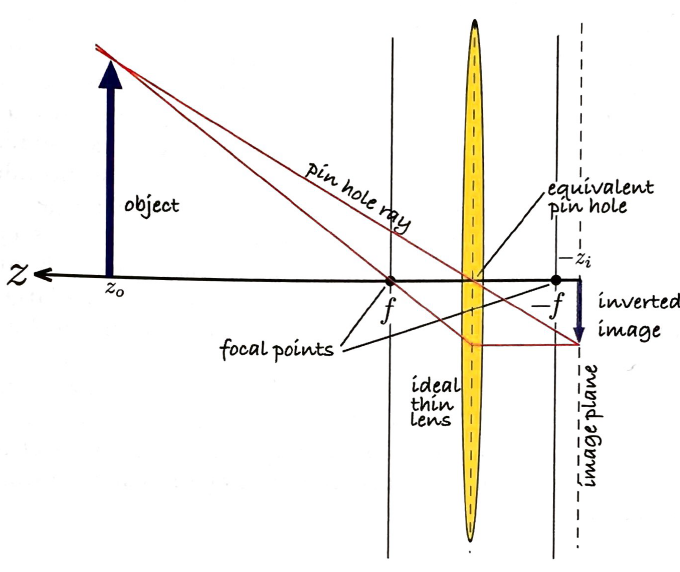
\includegraphics[scale=0.5]{./pics/imageFormationGeometry.png}
\caption{Image formation for a convex lens \cite{Corke}}
\label{fig:imageGeometry}
\end{center}
\end{figure}
The thin lens equation that describes the z-coordinate of the observed object and its image with respect to the CenterPoint of the image \cite{Corke}.
\begin{align}\begin{split}
&\frac{1}{z_0}+\frac{1}{z_i}=\frac{1}{f}\\
z_0&\text{ : the distance to the observed object.}\\
z_i&\text{ : the distance to the observed object.}\\
f&\text{ : is the focal length of the lens.}\end{split}
\end{align}
Its common in Computer vision engineering o use the center perspective imaging model  as shown in the following figure.
\\
%%problem displaying figure here
\begin{figure}[h]
\begin{center}
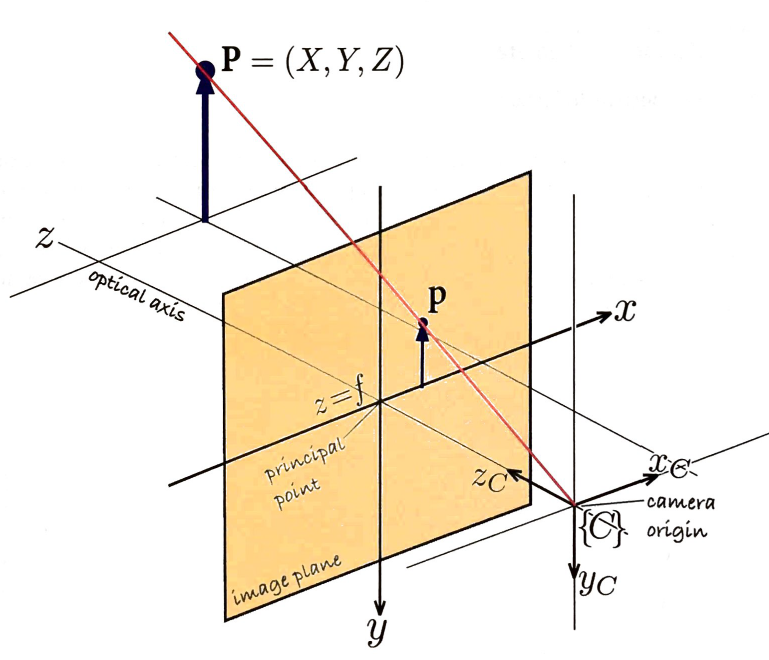
\includegraphics[scale=0.5]{./pics/CenterProjectionModel.png}
\caption{The central-projection model \cite{Corke}.}
\label{fig:projectionModel}
\end{center}
\end{figure}
\begin{subequations}
\begin{align}
\{C\}&\text{ : Origin of camera frame.}\label{eq:C_origin}\\
\textbf{P}=\left( X,Y,Z\right)&\text{ : Point in world coordinates.}\label{eq:P_w}\\
\textbf{p}=(x,y)&\text{ : Point on the image plane}\label{eq:P_i}
\end{align}
\end{subequations}
The rays of all corresponding Points \ref{eq:P_w} and \ref{eq:P_i} converge all at $\{C\}$ and a noninverted image is projected onto the image plane located at $z=f$ \cite{Ma:2010}. The z-axis intersects the image plane at the principal point which is the origin of the 2D image coordinate frame.
\begin{equation}
x=f\frac{X}{Z}, y=f\frac{Y}{Z}
\end{equation}

Through transformation from the world to image plane, the straight lines in the world are not projected as straight lines on the image plane, parallel lines converge and circles become ellipses, the size of a shape is not preserved and it depends on the distance.

\subsubsection{Modeling a perspective camera}
This sub--chapter refers to \cite{Corke}. By using the homogenous form $\tilde{\textbf{P}}=(\tilde{x} ,\tilde{y} ,\tilde{z} )$ to describe the image-plane point coordinates, where \begin{subequations}\begin{align}
&\tilde{x}=f\cdot X\label{eq:homo_x}\\
&\tilde{y}=f\cdot Y\label{eq:homo_y}\\
&\tilde{z}=Z\label{eq:homo_z}
\end{align}
\end{subequations}


are the homogeneous image-plane coordinate. As well we can formulate it in matrix form\cite{Corke}.
\begin{equation}
\tilde{\textbf{P}} = \begin{pmatrix}
f&0&0\\
0&f&0\\
0&0&1\\
\end{pmatrix}
\begin{pmatrix}
X\\
Y\\
Z\\
\end{pmatrix}
\end{equation}
and
\begin{align}
&x=\frac{\tilde{x}}{\tilde{z}}\\& y= \frac{\tilde{y}}{\tilde{z}}
\end{align}
are the nonhomogeneous image-plane coordinates.
\\
When $f=1$ the coordinates are referred to as the canonial, retinal or horizontalized image-plane coordinate and we can rewrite the homogenous coordinate like $ {}^{c}\tilde{\textbf{P}} = (X,Y,Z,1)^T $
then the perspective projection can be written in a linear matrix form like
\begin{equation}
\tilde{\textbf{P}} = C{}~^{c}\tilde{\textbf{P}}
\end{equation}

or the Camera matrix can be factorized into two matrices and the second matrix is the projection matrix 
\begin{equation}
\tilde{\textbf{P}} = \begin{pmatrix}
f&0&0\\
0&f&0\\
0&0&1\\
\end{pmatrix}\begin{pmatrix}
1&0&0&0\\
0&1&0&0\\
0&0&1&0\\
\end{pmatrix}{}^{c}\tilde{\textbf{P}}
\end{equation}

As known the camera will have an arbitrary pose $\varepsilon_c$ with respect to the world coordinate frame and can be shown and formulated as following 
\begin{figure}[h]
\begin{center}
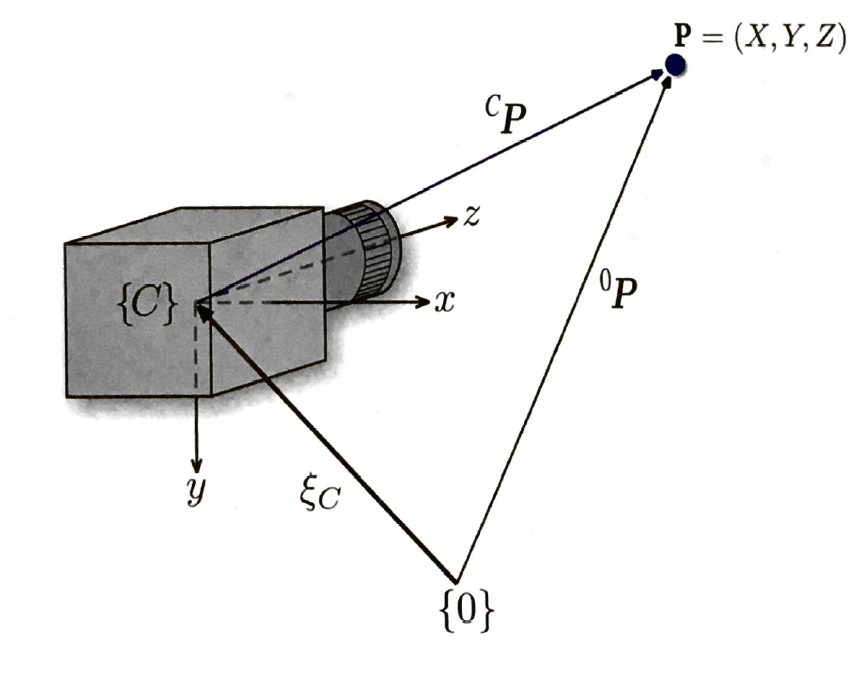
\includegraphics[scale=0.3]{./pics/cameraCoordinateFrame.png}
\caption{camera coordinate frame \cite{Corke}.}
\label{fig:cameraFrame}
\end{center}
\end{figure}

Or by using the homogenous coordinates 
\begin{equation}
{}^{c}\textbf{P}=\textbf{T}_c^{-1}\, {}^{0}\textbf{P}
\end{equation}

\subsubsection{Discrete image plane}
As shown on fig \ref{fig:projectionModel} the image plane in a digital camera constructed by $ W\times H $ photosites, which is light-sensitive elements, that correspond to pixels of the image.  The positive pixel coordinate system is a $2$--vector $(u,v)$ and the origin is at the top-left hand corner of the image plane.
The pixel coordinate is related to the image-plane coordinate by
\begin{equation}\frac{x}{\rho_w} + u_0, v = \frac{y}{\rho_h}+v_0\end{equation}
\begin{align*}
\rho_w&\text{ :  width of each pixel}\\
\rho_h&\text{  :  height of each pixel}\\
(u_0,v_0)&\text{  :  principal point}
\end{align*}

We can rewrite the linear perspective projection matrix in terms of pixel coordinates acknowledging the camera parameter matrix  $K$
\begin{equation}
\tilde{\textbf{P}}= \begin{pmatrix}
\frac{1}{\rho_w}&0&u_0\\
0&\frac{1}{\rho_h}&v_0\\
0&0&1\\
\end{pmatrix}\begin{pmatrix}
f&0&0&0\\
0&1&0&0\\
0&0&1&0\\
\end{pmatrix}{}^{c}\tilde{\textbf{P}}
\end{equation}

$\tilde{\textbf{P}}=(\tilde{u},\tilde{v},\tilde{w})$ : is the homogenous coordinate of the world p in the pixel coordinates
\begin{equation}
u= \frac{\tilde{u}}{\tilde{w}}, v= \frac{\tilde{v}}{\tilde{w}}
\end{equation}

$(u,v)$ : nonhomogenous image-plan pixel coordinates

\subsubsection{Camera matrix}
\label{sec:camMatrix}
From the previous equation the camera projection equation can be formulated in the general form as
\begin{subequations}\begin{align}
\tilde{\textbf{P}}&= \begin{pmatrix}
\frac{f}{\rho_w}&0&u_0\\
0&\frac{f}{\rho_h}&v_0\\
0&0&1\\
\end{pmatrix}\begin{pmatrix}
1&0&0&0\\
0&1&0&0\\
0&0&1&0\\
\end{pmatrix}{}^{0}\textbf{T}_c^{-1}\tilde{\textbf{P}}\\
\tilde{\textbf{P}}&= \textbf{K}\textbf{P}_0 \,{}^{0}\textbf{T}^{-1}_c\,\tilde{\textbf{P}}\\
\tilde{\textbf{P}}&= \textbf{C}\tilde{\textbf{P}}
\end{align}
\end{subequations}
Where the first two matrices are the intrinsic matrix and last two matrices are the extrinsic matrices.
The projection function can be written as\cite{Corke}
\begin{align}\begin{split}
\textbf{P}&=p(\textbf{P},\textbf{K},\varepsilon_c)\\
\textbf{K}&\text{ : camera parameter matrix}\\
\varepsilon_c&\text{ : camera pose}\end{split}
\end{align}
The camera Parameter matrix K includes the characteristics the camera and the sensors like $f,\rho,\rho_h,u_0$ and $v_0$. Furthermore, the pose of the camera holds the six extrinsic parameters that describe camera orientation and translation.
\\
There are a total of $11$ independent parameters to describe a camera, $5$ intrinsic and $6$ extrinsic parameters. In practical life, the camera parameters are not known and must be calculated by using a camera calibration process, which will be explained in the calibration section.
\\
The camera field of view is a function of its focal length f  and dimensions of the camera chip $W\rho_w  \times  H\rho_h$. The field of view can be determined from the geometry of fig \ref{fig:projectionModel}.
In the horizontal direction the angle of view is calculated as following.
\begin{align}
&\theta_h = 2\arctan{\frac{{W\rho}_w}{2f}}\\& \theta_v = 2\arctan{\frac{{H\rho}_h}{2f}}
\end{align}
\begin{align*}
W&\text{ : number of pixels in the horizontal direction}\\
H&\text{ : number of pixels in the vertical direction}\\
\rho_w&\text{ : width of a pixel}\\
\rho_h&\text{ : height of a pixel}\\
\end{align*}


\subsubsection{Lens Distortion}
As mentioned in the introduction, that no lens is perfect due to many factors. Lens imperfection leads to a geometric distortion, where points on the plane are not displaced where they should be.
\\
The geometric distortion is one of the most famous distortion effects that is comprises two components, the radial and tangential distortion. The Radial distortion is the displacement of the image points along radial lines from the principal point. The radial error can be approximated through the polynomial as following 
\begin{equation}
\delta_r=k_1r^3+k_2r^5+k_3r^7+...
\end{equation}
$r$ : is the distance of the image point from the principal point
The decentering distortion or the tangential distortion, occurs at the right angle to the radii but it's not stronger than radial distortion.
The can describe the coordinate of the distorted matrix as following 
\begin{equation}
u^d = u+\delta_u,v^d=v+\delta_v
\end{equation}
The displacement matrix is like the following, where the first matrix is describing the radial distortion and the second matrix describes the tangential distortion\cite{Corke}.
\begin{align}
\begin{split}
\begin{pmatrix}
\delta_u\\
\delta_v\\
\end{pmatrix}=\begin{pmatrix}
u(k_1r^2+k_2r^4+k_3r^6)\\
v(k_1r^2+k_2r^4+k_3r^6)\\
\end{pmatrix}+\\
\begin{pmatrix}
2p_1uv+P_2(r^2+2u^2)\\
p_1(r^2+2v^3)+2P_2uv
\end{pmatrix}
\end{split}
\end{align}
In practical life to describe the radial distortion only three coefficients are sufficient and the distortion model is parameterized by $(k_1,k_2,k_3,p_1,p_2)$. Which are considered as additional intrinsic parameters.

\subsubsection{Calibration with checkerboard}
\label{sec:checkerboard}
The calibration with a checkerboard is a popular toolbox for calibrating cameras by Caltech university. The images taken from the checkerboard have to be passed onto the toolbox uncompressedly. Since the default format of a USB Webcam is JPG, they first have to be converted to PNG format. For best results, 10 to 20 images have to be taken and the chessboard pattern has to be approximately 2 meters from the camera and has to cover as much of the image frame as possible as shown in the following figure.
%\begin{figure}[h]
%\begin{center}
%\includegraphics[scale=0.5]{./pics/chessboardOrientation.png}
%\caption{camera coordinate frame\cite{matlab}.}
%\label{fig:cameraCoordinateFrame}
%\end{center}
%\end{figure}


\begin{figure}[h]
\centering
\parbox{4cm}{
\includegraphics[width=4cm]{./pics/chessboardOrientation.png}
\caption{camera coordinate frame\cite{matlab}.}
\label{fig:cameraCoordinateFrame}}
\qquad
\begin{minipage}{4cm}
\includegraphics[width=4cm]{./pics/detectedPoints.jpg}
\caption{detected points with Matlab toolbox\cite{matlab}.}
\label{fig:detectedPoints}
\end{minipage}
\end{figure}


%\begin{figure}[h]
%\begin{center}
%\includegraphics[scale=0.10]{./pics/detectedPoints.jpg}
%\caption{detected points with Matlab toolbox\cite{matlab}.}
%\label{fig:detectedPoints}
%\end{center}
%\end{figure}
Moreover, a measurement of the exact length of one side of a square from the checkerboard pattern is necessary to improve the process accuracy. After passing the pattern images to the Toolbox, an image analyzing process starts to detect squares intersection points, checkerboard origin, and reprojected points.
To analyze each image, so it detects if the image is duplicated or if the entire chessboard could not be detected because of blurry images or an extreme angle of the pattern. After running the calibration,  The toolbox shows the different camera pose relative to the target for each calibration image.

\begin{figure}[h]
\centering
\parbox{4cm}{
\includegraphics[width=4cm]{./pics/cameraPoses.png}
\caption{camera poses for each calibration image~\cite{Corke}}
\label{fig:cameraPose}}
\qquad
\begin{minipage}{4cm}
\includegraphics[width=4cm]{./pics/meanErrorInPixel.png}
\caption{Reprojection Errors Bar Graph.}
\label{fig:ErrorsBarGraph}
\end{minipage}
\end{figure}

%\begin{figure}[h]
%\begin{center}
%\includegraphics[scale=0.2]{./pics/cameraPoses.png}
%\caption{camera poses for each calibration image\cite{Corke}.}
%\label{fig:cameraPose}
%\end{center}
%\end{figure}
Furthermore calibration accuracy can be evaluated by examining the fig.~\ref{fig:ErrorsBarGraph}. The bar graph displays the mean reprojection error per image, along with the overall mean error \cite{matlab} so images can be rejected for better calibration process.
%\begin{figure}[h]
%\begin{center}
%\includegraphics[scale=0.4]{./pics/meanErrorInPixel.png}
%\caption{Reprojection Errors Bar Graph.}
%\label{fig:ErrorsBarGraph}
%\end{center}
%\end{figure}

\subsection{Canny and Sobel edge detection}
\label{sec:Canny}
To perform camera calibration and to calculate the distortion for each pixel, so the camera will be stimulated with vertical and horizontal line at each position. However it's necessary for linedetection in a displayed image to cancel all environment noises so it's recommended to perform image processing like a \emph{gaussian}--blur to extract image primitives of interest \cite{opencv}. 
Lines could be extracted at regions where strong change of intensity or color in the processed Image is detected. In this section two different predefined line detection algorithms are compared and the second will be chosen, because it suits the requirements better\cite{Langaniere}.

\subsubsection{Sobel operator}
The main idea of the \emph{Sobel}--operator or \emph{Sobel}--filter is that it affects the vertical or horizontal image frequencies based on which kernel is used, therefore \emph{Sobel}--operator is considered as directional filter. On the other side \emph{Sobel}--operator is a gray scale operator so the image has to be converted to gray scale before applying the algorithm \cite{Langaniere}.
\\
The \emph{Sobel}--operator uses two Kernels that operates on each pixel that have the following form to calculate the derivatives of Intensity function \cite{Langaniere}.
\begin{equation}
Kernel_{vertical}=\begin{pmatrix}
-1&0&1\\
-2&0&2\\
-1&0&1\\
\end{pmatrix}
\end{equation}
\begin{equation}
Kernel_{horizontal}=\begin{pmatrix}
-1&-2&-1\\
0&0&0\\
1&2&1\\
\end{pmatrix}
\end{equation}
\begin{equation}
grad(I)=\begin{bmatrix}
\frac{\partial I}{\partial x},\frac{\partial I}{\partial y}
\end{bmatrix}^T
\end{equation}

%Sobel Figure

Since the calculated gradient lines at each pixel has a $x$ and $y$ direction, so it's interesting to calculate the norm and direction to get the amplitude of the variation and the orientation.
\begin{align}
&|grad(I)|=\sqrt[2]{\left(\frac{\partial I}{\partial x}\right)^2+\left(\frac{\partial I}{\partial y}\right)^2}\\
&\theta_{orientation}=\arctan{\frac{\partial I}{\partial y},\frac{\partial I}{\partial x}}
\end{align}
%Soble figutre Orientation 
The \emph{Sobel}--algorithm detects a lot of edges, which are not the actual edge because of the small kernel. Therefore the algorithm's results are noisy. 
\subsubsection{Canny operator}
The \emph{Canny}--operator is based on the output of the \emph{Sobel}--operator and it is very useful to remove the edges that aren't in interest. 
The \emph{Canny}--operator starts working on images after many stages. Firstly, the image should be converted to gray scale. After that the \emph{gaussian}--blur filter is applied \cite{opencv}. Hereafter the \emph{Sobel}--operator is applied on vertical and horizontal directions. At the end, the calculation of the orientation has to be done to get ready to apply \emph{Canny}--operator.
\\
The most powerful part of that method is the hysteresis thresholding. In the hysteresis thresholding there are two thresholdsd defined, $T_{min}$ and $T_{max}$. A search for an intensity value bigger than $T_{max}$ is started. If a pixel with such a high value is found the algorithm follows this border in both directions as long as a pixel value is higher than $T_{min}$. Every pixel that is found that way belongs to that border. If the complete image was searched for edges the algorithm is terminated. As a result, it provides an image of the dimension of the original image, in which only the edges are dyed white~\cite{opencv}.


\section{Mapping of correspondencing pixels}
\label{sec:mapping}
The aim of this project is to create a map of corresponding pixels of the screen to the camera image. To this end several different approaches has been tried which the accuracy in Chapter \ref{sec:results} and runtime in Chapter \ref{sec:runtime} are evaluated. \\
Before the mapping of the correspondences, the set-up of the device should be discussed. The camera should be in a distance to the screen that it only observes the screen and nothing else like the borders or so. The entire visible flat surface should be capable of manipulated by computer in order to excite every pixel on the camera image. The background color of the monitor should be black so that the drawn white pixels can be better recognized. The camera and the display should be in a locked dark area where no light is coming so the monitor is the only light source. This excludes the unwanted reflections that sophisticate the result. If the camera is adjusted perpendicular to the display the program could run.
\begin{figure}[h]
\begin{center}
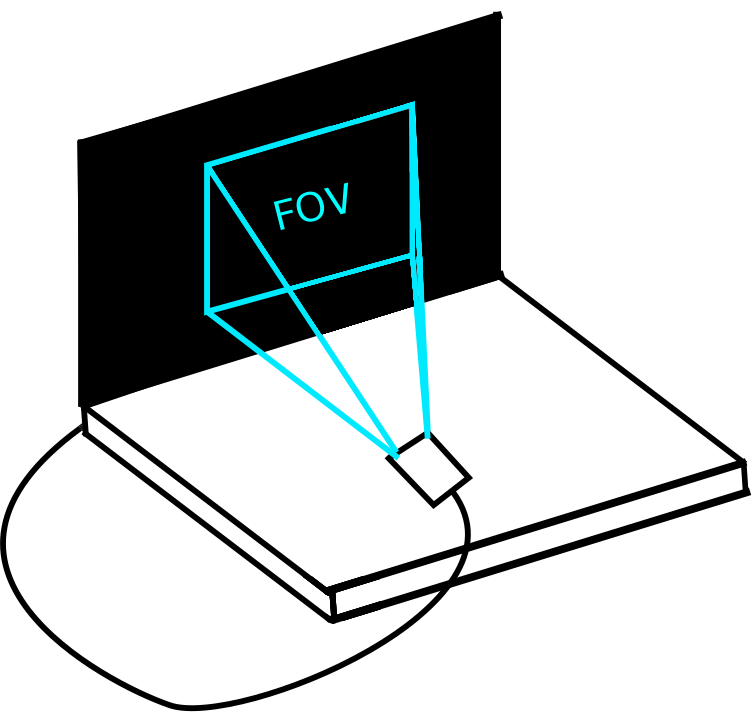
\includegraphics[scale=0.18]{./pics/setup.png}
\caption{Setup of Camera and Monitor}
\label{fig:setup}
\end{center}
\end{figure}\\
First is to be made sure, that the captured image contains at least one position at which the screen is going to display a rectangle. To this end a set amount of rectangles are drawn evenly spaced on the screen. Initially these rectangles have a \emph{width} and \emph{height} of $1$. While the camera doesn't detects a pixel, the \emph{width} and \emph{height} of the drawn rectangle should be increased by $1$ until it does recognise a drawn pixel. This is shown in algorithm~\ref{algo:pixelsize}.
\begin{algorithm}[h]
 \KwData{cameraImage}
 \KwResult{returns pixelSize}
 initialization: int pixelSize = 1\;
 \While{(notDetected)}{
  \eIf{(maxBrightnestPixel != 0)}{
   notDetected = false\;
   return pixelSize\;
   }{
   notDetected=true\;
   pixelSize++\;
  }
 }
 \caption{pixel size detection}
 \label{algo:pixelsize}
\end{algorithm} 
 In order to ensure, that the detection was not a accidental chance of luck, the same size has to be confirmed by further detections. \\
After the pixel size which can be seen by the camera is detected, a pixel with that size is drawn on the screen which is moving with a spacing. That means that the pixel always gets a new coordinate that with a calculated distance in vertical and/or horizontal  direction. Therefore it's possible to calculate an optimal spacing for a specific method which is described at the end of Chapter \ref{sec:linebased}. While the pixel is moving on the screen the $x_s$ and $y_s$ positions of the seen rectangles on the screen are accumulatively added. Simultaneously the number of seen rectangles is enumerated. The algorithm is shown in~\ref{algo:centerPoint}.\\
As shown in the following chapters, these two methods are fundamental to most of the approaches. While the pixelSize is not necessary for the algorithm itself, it will still be used to generate a test image. To this test image the found distortion maps are applied. Therefore they are necessary in any case. In the next three sub-chapter two principle different possibilities are presented. These could be possible methods to get a distortion calibration with a higher accuracy than the state of the art. 
 
\begin{algorithm}[h]
 \KwData{pixelPosition}
 \KwResult{returns centerPoint}
 initialization: int counter = 0\;
 \While{(pixelPosition < display)}{
  \eIf{(pixelSeen)}{
   centerPoint += pixelPosition\;
   counter++\;
   }{
   centerPoint /= counter\;
   }
 }
 \caption{calculation of center point of FOV}
 \label{algo:centerPoint}
\end{algorithm} 

\subsection{Pixelwise approaches}
The idea was a matching from every screen pixel to his corresponding pixel in the image. Three different methods are developed. These were faster in their implementation in this order, with the same accuracy. The duration of the individual methods is given in Chapter \ref{sec:runtime} with an exact minimum value for the given example.
\subsubsection{Enlighting every Pixel}
The first and easiest idea is to light a rectangle with minimum pixel size after another and row for row. If a drawn rectangle is detected by the camera, then save the correspondences of the image and the screen coordinate. It can be checked if an imaginary straight line of rectangles on the screen will be to a straight line of pixels on the image. If not, then the next step is to move the image pixels until the line seen on the image is also straight.
\subsubsection{Moving the pixel in spiral shape}
However it's not very efficient by lighting every pixel of the screen with the seen pixel size. As the seen area on the screen the field of view (FOV) could be significant smaller than the screen another method was developed to ensure a faster result. For this purpose  the rectangle is moved on a spiral-like path on the screen. The algorithm \ref{algo:centerPoint} was designed to find a optimal starting position to that spiral. After finding the center point of the FOV the rectangle moved slowly to the outside of the FOV. While the pixel wasn't seen for a hole circulation it's sure that the rectangle moved out of vision of the camera. So each time a rectangle is detected, it's position on the screen and the camera image will be saved for the distortion calibration later on. Exposing the view area in spiral-shape, as described in Chapter \ref{sec:runtime}, is not exactly fast. In addition, the method is very inefficient for fish-eye cameras or any kind of wide angle cameras. 

%% mathematics and basics -> some pictures with different distortion shapes
\subsubsection{Linebased approach after borderdection}
\label{sec:boderDetect}
The pixel-wise distortion calibration was the last concept in which was tried to detect a solution by lighting several rectangles with the minimum pixel size. However this method is already a hybrid since the real line detection methods are introduced here to solve the problem of distortion calibration. In the further discussed methods the pixel correspondence is used and the lines in both images (the drawn and the detected one) are calculated. In this method lines are drawn in the seen area and their position in the camera image are detected and later be corrected. However the borders of the seen area should first be detected. To this end it is forced to find at least one border of the seen area. Therefore a binary search algorithm is developed in order to find a border. The initial point to that algorithm is the center point which has been already detected with algorithm~\ref{algo:centerPoint}. From there it is assumed that a point at any border of the screen is not seen by the camera. Then it will be checked if a point between this two points is seen or not. If not then check between this and center point or else check between that and the point of the border. %This is described in algorithm~\ref{algo:binary}. 


%\begin{algorithm}[h]
% \KwData{pixelPosition}
% \KwResult{returns borderPoint}
% initialization: \;
% point lastSeen = centerPoint\;
% point lastNotseen = screenBorder\;
% point nextPos\;
% \While{(abs(lastSeen - lastNotSeen)>1)}{
% nextPos = (lastSeen+lastNotSeen)/2\;
%  \eIf{(pixelSeen)}{
%   lastSeen = pixelPosition\;
%   }{
%   lastNotSeen = pixelPosition\;
%   }
% }
% pixelPosition = nextPos\;
% return borderPoint = (lastSeen+lastNotSeen)/2\;
% \caption{binary search algorithm for border detection}
% \label{algo:binary}
%\end{algorithm} 

In the process of this work the binary search showed that absolute darkness around the setup is necessary because otherwise in the outer area of the camera image pixels that could be seen aren't seen. \\
After a border is found, the next step is to find all corresponding screen pixels which belongs to the frame of the camera image. If these are found, then draw lines with \emph{width} for vertical lines and the \emph{height} for horizontal lines of the minimum pixel size on the screen that are straight. Then it is possible  to calibrate the distortion with the next two shown images. However, it could still need a long time to detect the borders since around a pixel, it exists 8 possible positions to detect the next one that belongs to the frame. Even if some of these possible positions can be excluded if the side of border and the direction of movement are known, at least 4 possible positions still remain. \\%% Picture Positions? 
In Chapter \ref{sec:runtime} the minimum time required for an exemplary FOV is calculated. However this method was dismissed too because a way faster solution with a line detection by a \emph{openCV}--function called \emph{Canny} was found. 

\subsection{Simple linedetection for mapping}
\label{sec:linedetect}
\begin{figure}[h]
\centering
\parbox{4cm}{
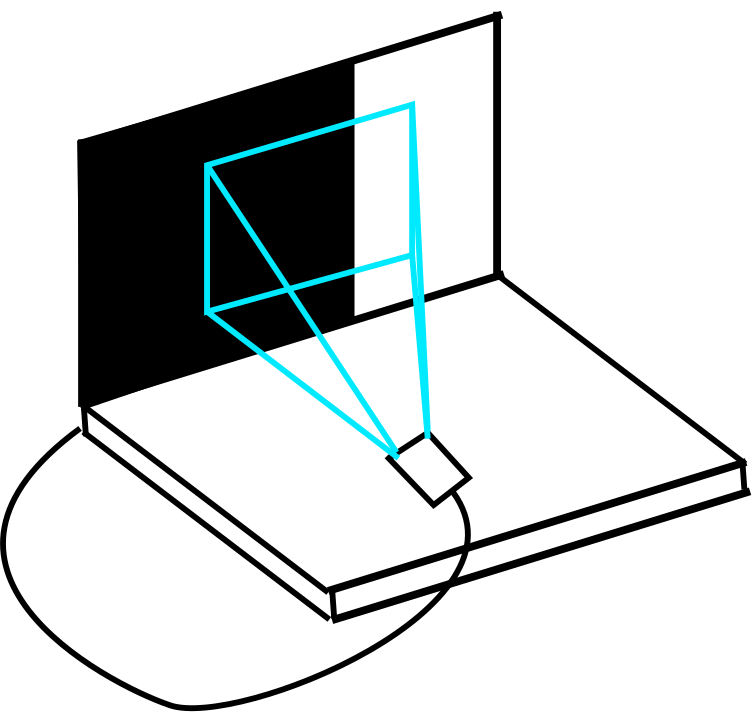
\includegraphics[width=4cm]{./pics/rect.png}
\caption{Rectangle moving over the screen}
\label{fig:setup}}
\qquad
\begin{minipage}{4cm}
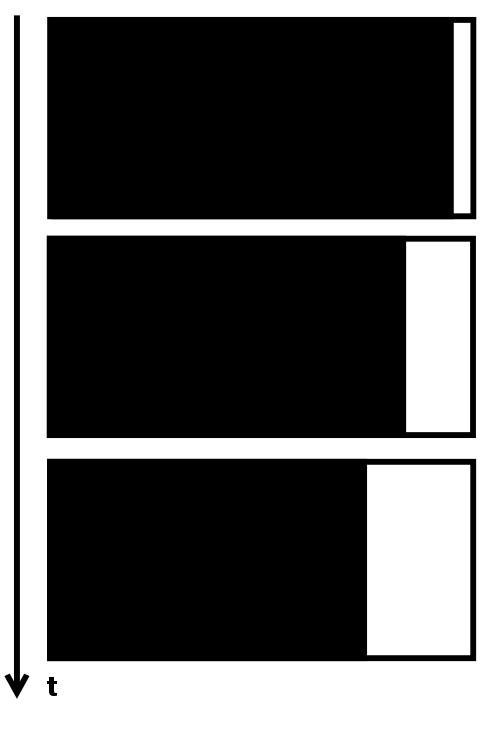
\includegraphics[width=4cm]{./pics/pattern.png}
\caption{Rectangle over time}
\label{fig:blockOverTime}
\end{minipage}
\end{figure}


The background of the screen is set to be black. Then a white rectangle with height of the screen height is drawn, which has a increasing width. In figure \ref{fig:blockOverTime} how the rectangle is getting wide is shown. At the border of the white rectangle to the black background the \emph{Canny}-operator detects the points of the border as a line. The return of that operation is a point cloud of image coordinates that belong to that line. To every image pixel that in that point cloud the $x$--coordinate to which it should belong is matched. The width of the rectangle is enlarged until it disappears from the FOV.\\
After that the rectangle is generated from up to down with the same method. Every pixel that belongs to that line in a point cloud by the \emph{Canny}--operator will also be obtained. Now the $y$--coordinates to the points which are obtained can be matched, since they always belong to the actual drawn line. At the end of Chapter \ref{sec:runtime} the runtime of this method is calculated .\\
It is significantly faster than any of the other methods that were presented so far. However, it can be accelerated even more, if several instead of one pixel size is set as step. To obtain a dense image, a interpolation function is written that interpolates linearly between matched pixels. In future it could be tested if another interpolation method besides linear interpolation give better results. In case of radial distortion a radius to the center point dependent interpolation could return better results.\\

\subsection{Runtimes and Field of View}
\label{sec:runtime}
\subsubsection{Field of View}
\label{sec:FOV}
Each frame makes one call to the draw function. Given that it need $7$ calls of the draw function to fully draw, capture, and process one image. With a frame rate of $21$ frames per second a turnover rate of $3$ images per second is achieved. This allows to make an estimation of the runtime of each approach that was tested out or considered for the lens calibration based on the amount of necessary images. The runtime $rt$ of the program could be calculated as shown in the following Chapter. 
\begin{align}
rt(noImages) = \frac{1}{3} \cdot noImages 
\end{align}
To determine the amount of images for some methods an estimate of the field of view is needed. In order to estimate the FOV a simple method with a measuring tape was used. The only further information necessary, is the amount of pixels per inch ($ppi$) of the used screen. By placing the measurement tape flat on the screen it's possible to measure the width and height that are visible in the captured image. The measurement then has to be converted to inches in order to calculate the amount of pixels. The conversion constant from centimeters to inches is roughly $0.3937$. Multiplying this with the ppi yields the pixels seen. Let $l$ be the length of the visible measurement tape in centimeters, then the amount of pixels in the FOV can be calculated as:
\begin{align}
FOV(l) = ppi \cdot 0.3937 \frac{inch}{cm} \cdot l .
\end{align}
From there it's possible to calculate the diagonal aperture angle of the camera. By comparing the calculated angle with the angle from the specifications of the camera, we have an estimation about the accuracy of the calculated FOV. If the diagonal aperture angles differ largely, the estimation is inaccurate. If they are similar, it is acceptable.\\
To calculate the aperture angle $\alpha$ for the width or height $\left( \alpha_{width||height}\right)$, the distance $d$ of the camera to the screen is needed too. The distance and FOV dimensions need to be used with the same unit. From there the aperture angle is simple trigonometry, see image \ref{fig:dist}.


\begin{figure}[h]
\begin{center}
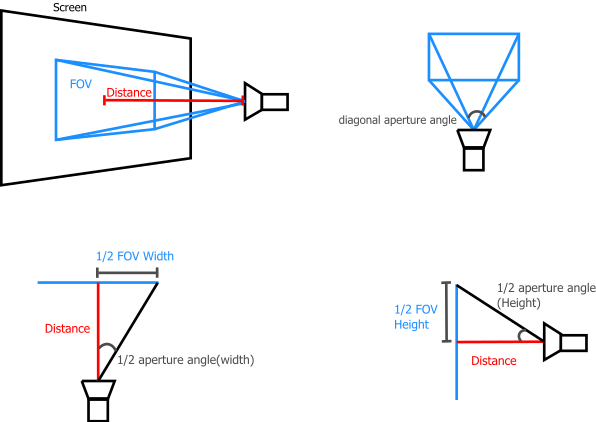
\includegraphics[scale=0.4]{./pics/distanceandangles.png}
\caption{Distance and angles of the FOV}
\label{fig:dist}
\end{center}
\end{figure}



\begin{align}\begin{split}
&\frac{1}{2}\cdot\alpha_{width||height}  =  \arctan \left(\frac{FOV_{width||height }}{2\cdot d} \right),
\end{split}
\end{align}
\begin{align}\begin{split}
\Rightarrow &\alpha_{width||height} = 2 \cdot \arctan \left(\frac{FOV_{width||height }}{2\cdot d} \right),
\end{split}
\end{align}
\begin{align}\begin{split}
&\alpha_{diag} = \sqrt{\alpha_{width}^2 + \alpha_{height}^2)}.
\end{split}
\end{align}
In the setup an \emph{ASUS--VX239} screen of dimensions $1290$x$1080$ pixels and $95.78~ppi$ and a \emph{Microsoft~LifeCam~HD--3000} was used. To place the camera exactly perpendicular to the screen wasn't possible as the results showed. This warps the FOV somewhat. Therefore an average of the largest and smallest measurement of the FOV width and height is used. On average a width of $17.75~cm$, and a height of $10.45~cm$ was measured. This yields the FOV dimensions to
\begin{align*}
FOV_{width}(17.75~cm) \approx 669.327~pixels
\end{align*}
\begin{align*}
FOV_{height}(10.45~cm) \approx 394.050~pixels
\end{align*}
Since to rather overstate the runtime than understate it, $670$ pixels for the width and $395$ for the height are used. The distance between camera and screen was roughly $16.0~cm$. This yields aperture angles of:
\begin{align}\begin{split}
\alpha_{width}(17.75~cm)&= 2 \cdot \arctan\left(\frac{17.78~cm}{2 \cdot 16~cm}\right) \\&= 58.12^{\circ}\end{split},
\end{align}
\begin{align}\begin{split}
\alpha_{height}(10.45~cm) &= 2 \cdot\arctan\left(\frac{10.45~cm}{2 \cdot 16~cm}\right) \\&= 36.17^{\circ}\end{split},
\end{align}
\begin{align}\begin{split}
\alpha_{diag} &= \sqrt{58.12^2 + 36.17^2} \\& \approx 68.46^{\circ}.\end{split}
\end{align}
The specifications for the camera state a diagonal aperture angle of $68.50^{\circ}$. Judging from the difference of roughly $0.04^{\circ}$, this should be close enough to the true FOV dimensions to use it for runtime estimations.Furthermore the assumption is made that each pixel can be detected on its own, instead of needing larger patches to be detectable by the camera.\\
The following variables will be use: $h_{FOV}$ as the height of the FOV, $w_{FOV}$ as the width of the FOV, $w_s$ as the width of the screen, and $h_s$ as the height of the screen.\\
\subsubsection{Pixelwise detection}
\label{singlePixel}
With a naive approach each patch of minimal detectable size on the screen has to be turned on separately.
\begin{align}
rt(w_s, h_s) = \frac{1}{3} \cdot w_s \cdot h_s
\end{align}
This means screen width times screen height necessary images. In this set up $921,600$ images would be needed, yielding a runtime of $307,200$ seconds ($sec$), or $3$ days $13$ hours $20$ minutes ($min$).\\
It can be sped up however. By lighting up single pixels in a spiral pattern around an estimation of the middle point, the amount of images can be reduced to the amount of pixels within the camera’s FOV plus one pixel in each dimension. The additional pixel is necessary, because it allows to know, when the spiral does not need to actually be done, but can jump to a next position. This is due to the pixel outside no longer being detected. \begin{align}
rt(w_{FOV}, h_{FOV}) = \frac{1}{3} (w_{FOV} + 1) \cdot (h_{FOV} + 1)
\end{align}
In the setup, $265,716$ images were needed, leading to a runtime of $88,572$ $sec$, or $1$ day $36$ hours $12$ $sec$. The center point estimation has been left out, as it is comparably negligible.\\
	
\subsubsection{Line-based detection} 
\label{sec:linebased}
In this subsection the runtime of the method of section \ref{sec:boderDetect} is calculated.
\begin{align}
rt(w_{FOV}, h_{VOF}) = \frac{4}{3} (2 \cdot h_{FOV} + 2 \cdot w_{FOV})
\end{align}
In this setup, $8,520$ images are needed, leading to a runtime of $2,840$ $sec$, or $47$ $min$ $20$ $sec$, only for the border detection. After discovering the border only two images need to be created and processed. However, since the discovery of the border would take still too long, this method was rejected as well.\\
The next method is a segmentation of the screen. By segmenting the screen sequentially in a black and a white part, a single edge could be detected in the image. The white part starts out as the entire screen and gradually decreases in width, pixel by pixel. After that is done, the white part is again stretched out over the entire screen and then decreases in height. At each image the exact position where the screen shows the edge is known. From there a calculation where the edge pixels from the image should have appeared is possible.\\
A naive and simple approach is to go along the entire screen width and height. Each row and each column is once the edge row or column. This leads to a runtime of
\begin{align}
rt(w_s, h_s) = \frac{1}{3} (w_s + h_s)
\end{align}
In this setup state,  $2,370$ images are needed, leading to a runtime of $790$ $sec$, or $13$ $min$ $10$ $sec$.  This is already immensely faster. It can still be sped up, however.\\
Instead of going over the entire screen an estimation of the center point is done again. This time additionally the outermost pixels, which was visible during the estimation, are stored for each border. From there the spacing is added, that was used, plus a small margin to be safe. The margin was chosen to be $5$ pixels wide. In this method the runtime for the center point estimation is relevant. While the runtime for the center point estimation increases with smaller spacing, the runtime for the line-based detection decreases. This means a runtime-optimal spacing can be calculated.\\
Let $s$ be the spacing between the positions of the pixels to be lit, and $m$ the margin. Then the runtime of the center estimation $rt_c$, as a function of spacing $s$, is:
\begin{align}
rt_c (s) =\frac{1}{3} \frac{w_s\cdot h_s}{ s^2} =\frac{1393200}{3s^2} .
\end{align}
For the runtime of the line-based detection after that, follows:
\begin{align}\begin{split}
rt_d (s) &=\frac{1}{3}\left( 4s + 4 m + w_{FOV} + h_{FOV}\right)\\& = 4s + 1085\end{split}
\end{align}
From there the overall runtime can be calculated as:
\begin{align}\begin{split}
rt(s) &=\frac{1}{3}\left(\frac{w_s h_s}{s^2} + 4s + 4m + w_{FOV} + h_{FOV}\right)\\& = \frac{\frac{1,393,200}{s^2} + 4s +1085}{3}.\end{split}
\end{align}
For calculating the minimum of this function the first derivative is taken and the w.r.t. spacing $s$ is set to $s=0$:
\begin{align}\begin{split}
&rt’(s) = \frac{1}{3} \cdot \left( \frac{-w_s \cdot h_s}{s^3 }  + 4\right) = \frac{ \frac{-1,393,200}{s^3}+ 4}{3},\\
\Rightarrow &s = \sqrt[3]{\frac{w_s  h_s}{4}} = \sqrt[3]{\frac{1393200}{4}}. \end{split}
\end{align}

The functions minimum is at roughly $s = 70$. For this spacing $1,650$ images are needed wjch is leading to a runtime of $550$ $sec$, or $9$ $min$ $10$ $sec$. Of these roughly $1$ $min$ $35$ $sec$ are taken by center point estimation.\\
If this is deemed too slow, but the restriction of true pixelwise mapping is lifted, it can be sped up. If an amount of pixels is skipped, when moving the white rectangle over the screen. The jump width is introduced as variable $j$, i.e. every $j$--th pixel will be part of an edge. This changes the runtime formula for the detection part too, when assuming the same margin $m$:
\begin{align}\begin{split}
rt_d (s; j) &=\frac{1}{3} \cdot \frac{4s + 4  m + w_{FOV} + h_{FOV}}{j}\\
 &= \frac{4s + 1085}{3j},\end{split}
\end{align}
and thus the overall formula and its derivative to:
\begin{align}\begin{split}
rt(s; j) &= \frac{1}{3} \left(\frac{w_s\cdot h_s}{3} + \left( 4s + 4m + w_{FOV} + h_{FOV}\right)\frac{1}{j}\right)\\ &=\frac{1}{3}\left( \frac{1,393,200}{s^2} + \frac{4s +1085}{j}\right),\end{split}
\end{align}
\begin{align}\begin{split}
rt’(s; j) &= \frac{1}{3} \left(\frac{-w_s \cdot h_s}{s^3} + \frac{4}{j}\right)\\& =\frac{-1,393,200 }{3s^3} + \frac{4}{3j} \end{split}
\end{align}
The new optimal spacing is now calculated as:
\begin{align}\begin{split}
s &= \sqrt[3]{\frac{w_s \cdot h_s \cdot j }{ 4}} \\&= \sqrt[3]{\frac{1,393,200 \cdot j} { 4}}.\end{split}
\end{align}
For a skip of $j = 3$ in that setup an optimal spacing of roughly $s = 101$ is optimal. For this spacing and skipping only $633$ images are necessary leading to a runtime of $211$ $sec$, or $3$ $min$ $31$ $sec$. Of these roughly $46$ $sec$ are taken by center point estimation.




\section{Results}
\label{sec:results}
In this chapter the results of the presented method in section \ref{sec:linedetect} are shown. The results of a commonly used method was shown in \ref{sec:checkerboard} as the calibration with a checkerboard. There in fig. \ref{fig:ErrorsBarGraph} a accuracy with a \emph{mean} of $1.24$ pixels is reached. At first the accuracy that is reached threw mapping is shown. Then the results are compared and evaluated.
\subsection{Accuracy}

The accuracy of the method depends on the precision of the edge detector and the jump width. The larger the range, the further the distance that has to be interpolated between two seen pixels. Since, as mentioned in the following chapter, no other interpolation algorithms have been tried, it is not conclusive to say to what extent this contributes to inaccuracies. With a jump range of $1$ pixel size the deviation of the mapped image compared to ground truth is with $846$ pixel errors with $294,480$ a total perceived pixels. This leads to $0.287\%$ incorrect placed pixels in the hole image.

\begin{figure}[h]
\centering
\parbox{4cm}{
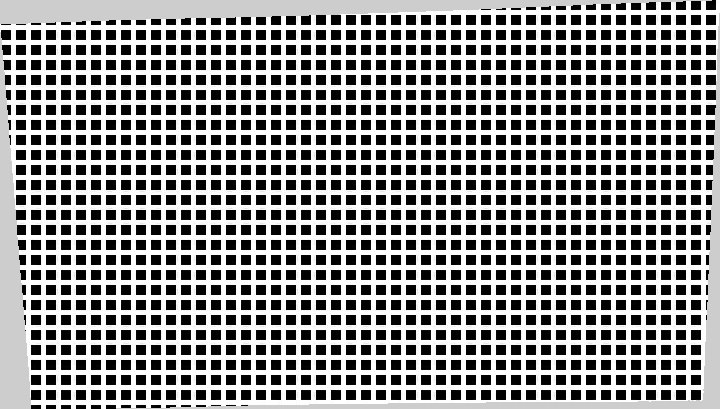
\includegraphics[width=4cm]{./pics/gt.jpg}
\caption{Ground truth}
\label{fig:gt}}
\qquad
\begin{minipage}{4cm}
\includegraphics[width=4cm]{./pics/seenImage.jpg}
\caption{mapped image}
\label{fig:undistImage}
\end{minipage}
\end{figure}



\subsection{Comparison and evaluation}
\label{sec:conclusion}
For evaluation the mapping was tested with several jump distances: $1$, $3$ and $5$ pixel size. With jump range the percentage of deviated pixels was $0.287\%$. With range of $3$ pixel size the deviation increased by $10.45\%$ to $0.317\%$. At jump range of $5$ the deviation increases to $0.398\%$. 

\begin{figure}[h]
\begin{center}
\includegraphics[width=8cm]{./pics/withAlignment.jpg}
\caption{Difference: ground truth to undistorted image\\ white spots results from difference}
\label{fig:diff}
\end{center}
\end{figure}

As seen the most different pixels are in the center. This is because the black and white area must be flipped there. If the white area becomes noticeably smaller, the edge is no longer recognized by Canny. For this reason, the areas are flipped in order to recognize the edge continuously. 

To compare this with other methods the \emph{Stdev} of a pixel was calculated. This deviation should be roughly $0.81\mu m$. This is better than any other method proposed in \cite{Salvi}.

\section{Future work and problems}
\label{sec:work_probs}
In this section the problems with the \emph{openframeworks} and openCV Libraries that occured during this work are presented in \ref{sec:probs}. After that, ideas and possible improvements are introduced in \ref{sec:future}, which could not be implemented anymore.
\subsection{Problems}
\label{sec:probs}
Several problems appear during the process of this project.
The first is the use of new programming tools. \emph{Openframeworks} is a toolkit with powerful embedded functions (setup(), update() and draw()) which has an advantage that draws parallel to processing, however, it brings timing issues into the project, since the update function only runs once before drawing. Getting rid of it costs the first several weeks and slowed the process down. Ultimately each app was divided into several states in draw(), and use a state machine to control the process, which turns out to be a good solution.  \\
The next problem is, several classes with their own functions has been written to achieve a modularly structured program. A  master--class was created to bring these module--classes and their functionality together. So each module--class brings a functionality and together they solve the given problem to undistort a image. This splitting of the code made it necessary to retain information gained in each part. This, however, was a problem. Any class that is supposed to draw on the screen, needs to inherit from \emph{openframeworks} class ofApp. Any class that inherits from class ofApp, has to be started with the \emph{openframeworks} function ofRunApp.\\
While the runtime of each App, the only way to access data is to work with multi-threading and trying to access variables from another thread. Since it have to be ensured, that there are no read~/~write access violations and that the threads are properly synchronized, this method is problematic. \\
There is also a problem to access information after the runtime of the apps, since after the runtime of the app all variables used within are deleted. To overcome this disadvantage, a pointer of the app is introduced to a variable outside of it. This ensured that the app wrote into that variable. Since the variable wasn't within the scope of the app, the information in it was retained even after the app was closed and deleted.\\
The modular program structure was important, as an overview of the code could be lost else. It also allows functionalities easily replaceable as long as the defined interfaces are kept the same.
\\
It was necessary to set ofSetBackgroundAuto(false) to avoid flickering of the screen, which brings problematics for Win10 systems because of incompatibility. On Win7 this functionality runs without problems. \\
Also it's necessary to run the program in two steps because to load and save images isn't possible while \emph{ofBaseApp} of \emph{openframeworks} was running. In the \emph{openframeworks} the functions still not work at version $0.9.8.vs\_release$.


\subsection{Future work}
\label{sec:future}
The first step in the future work should be that the undistortion runs in one step. Therefore some bugfixes by the \emph{openframeworks} team itself are necessary or a workaround should be found. Like already told in section \ref{sec:linedetect} the results should be valuated if a radial interpolation maybe leads to a better result of the mapping itself. At the moment the solution is running with a global variable that sets the threshold for a detected pixel. This was estimated empiric. This could be replaced by a function that enlarge a seen white pixel until a pixel in that is seen with the white real white value of $255$. In the moment the \emph{Canny}--operator is used to detect edges however also this maybe could improved too. Therefore a idea is to draw a horizontal line threw the center point that was detected and then all the other lines. With or without jump of pixels. The position of the center line is known by what the for each line the position of a line could be detected by evaluate the intensity value. Since a pattern is drawn a distorted pattern should be detected. So the fourth line should be still the fourth line in the image. This method maybe runs even faster since with \emph{Canny} every line has to be drawn single. With this method only $4$ images are needed. The horizontal and vertical center line and then all the other lines. Also with \emph{Canny} there are problems while the flipping of the rectangles, told in section~\ref{sec:conclusion}.
After that also the mapping method could be improved because it sometimes maps reflections into the image. So pixels are seen at a place where none are possibly detected.
At least maybe once the statemachine isn't necessary any more and the developed architecture isn't necessary so the update() function of \emph{openframeworks} could be used.  

%\bibliography{literatur}

\begin{thebibliography}{1}
\bibitem{Zhang}
Zhang and Zhengyou. \emph{A flexible new technique for camera calibration}, p.965--980, vol.14 num.10, IEEE Transactions on Pattern Analysis and Machine Intelligence, 2010

%\bibitem{Sturm}
%P.F.~Sturm and S.J.~Maybank. \emph{On plane-based camera calibration: A general algorithm, singularities, applications}, Computer Vision and Pattern Recognition, IEEE Computer Society Conference on. IEEE, p.432--437, 1999

\bibitem{Faugeras}
O.~Faugeras, Q.T.~Luong and S.~Maybank. \emph{Camera self-calibration: Theory and experiments},p. 321--334Computer Vision--ECCV'92, 1992

\bibitem{Ma:2010}
Y.~Ma. \emph{{An invitation to 3-D vision: From images to geometric models}, {Springer} , {978-1-4419-1846-8}}

\bibitem{Sagawa}
R.~Sagawa and M.~Takatsuji and T.~Echigo and Y.~Yagi . \emph{Calibration of lens distortion by structured-light scanning} IEEE/RSJ International Conference on Intelligent Robots and Systems, p.832--837 , 2005

\bibitem{Salvi}
J.~Salvi and J.~Pag{\`e}s and J.~Batlle. \emph{Pattern codification strategies in structured light systems}, vol.37 num.4, Pattern Recognition, p. 827--849, 2004

\bibitem{Swaminathan}
R.~Swaminathan and S.K.~Nayar. \emph{Nonmetric calibration of wide-angle lenses and polycameras}, p.1172--1178, vol.22 num.10, IEEE Transactions on Pattern Analysis and Machine Intelligence

%\bibitem{Weng}
%J.~Weng and P.~Cohen and M.~Herniou. \emph{Camera calibration with distortion models and accuracy evaluation}, p.965--980, vol.14 num.10, IEEE Transactions on Pattern Analysis and Machine Intelligence, 1992

\bibitem{Duane}
C.B.~Duane  \emph{Close-range camera calibration}. Photogramm. Eng, vol.37 num.8, p.855-866. 1971

\bibitem{Corke}
C.B.~Peter Corke  \emph{Robotics, Vision and Control: Fundamental Algorithms In MATLAB® Second, Completely Revised, Extended And Updated Edition }. Eng, vol.1 , p.319-356. 2017

\bibitem{Langaniere}
C.B.~Robert Laganiere  \emph{OpenCV3 ComputerVision Application Programming Cookbook }. Eng, vol.3, 2017

\bibitem {Wikipedia}
WIKIPEDIA {The Free Encyclopedia}
\url{https://simple.wikipedia.org/wiki/Pinhole_camera} 06.07.2017\\
\url {https://en.wikipedia.org/wiki/Distortion_(optics)} 07.07.2017.\\
\url {https://en.wikipedia.org/wiki/Canny_edge_detector} 07.07.2017.\\
\url {https://en.wikipedia.org/wiki/Sobel_operator} 07.07.2017.
\bibitem {opencv}
OPENCV {Open Source Computer Vision Library}
\url {http://docs.opencv.org/2.4/doc/tutorials/imgproc/imgtrans/canny_detector/canny_detector.html} 20.06.2017.\\
\url {http://docs.opencv.org/2.4/doc/tutorials/imgproc/imgtrans/sobel_derivatives/sobel_derivatives.html} 20.06.2017.\\
\url {http://docs.opencv.org/2.4/doc/tutorials/calib3d/camera_calibration/camera_calibration.html} 15.06.2017.\\
\bibitem {matlab}
MATLAB {MathWorks}
\url {https://www.mathworks.com/help/vision/ug/single-camera-calibrator-app.html}
\end{thebibliography}

\begin{biography}[{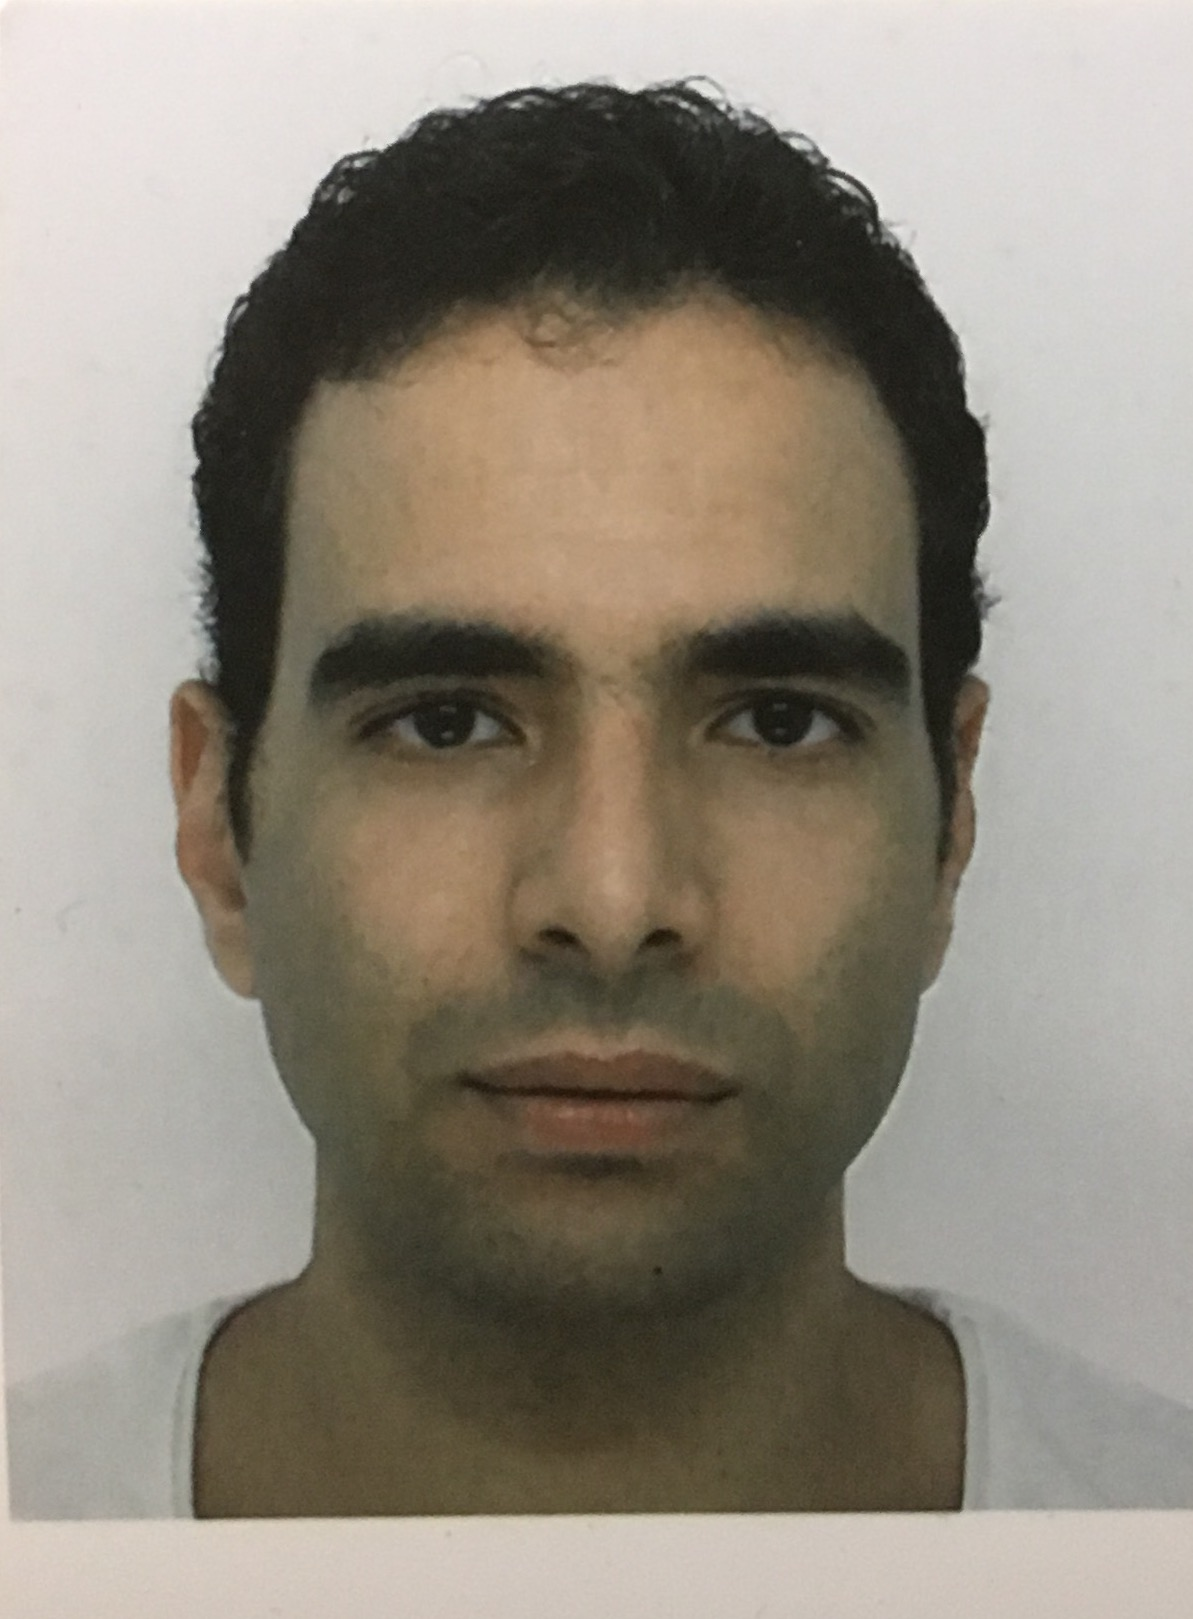
\includegraphics[width=1in,height=1.25in,clip,keepaspectratio]{./pics/FullSizeRender.jpg}}]
{Ahmed Ashraf Mohammed} received his B.~Sc. in Mechatronic at TU--Darmstadt in 2016.
His B.~Sc. Thesis was about optimization of rotating moment of pick and place robot. Since 2016 he is studying MSc. Mechatronics with specialization on Simulation and Control at TU--Darmstadt.
\end{biography}
\begin{biography}
[{\includegraphics[width=1in,height=1.25in,clip,keepaspectratio]{./pics/passbild.jpg}}] % hier ein Foto einbinden
{Nils Hamacher} received his B.~Sc. in EtIt at TU--Darmstadt in 2016. His Thesis was about an optimization of a center line calculation by 2 borders of a racetrack. Since 2016 he is studying M.~Sc. EtIt with specialization in Automatisierungstechnik at TU--Darmstadt.
\end{biography}
\begin{biography}
[{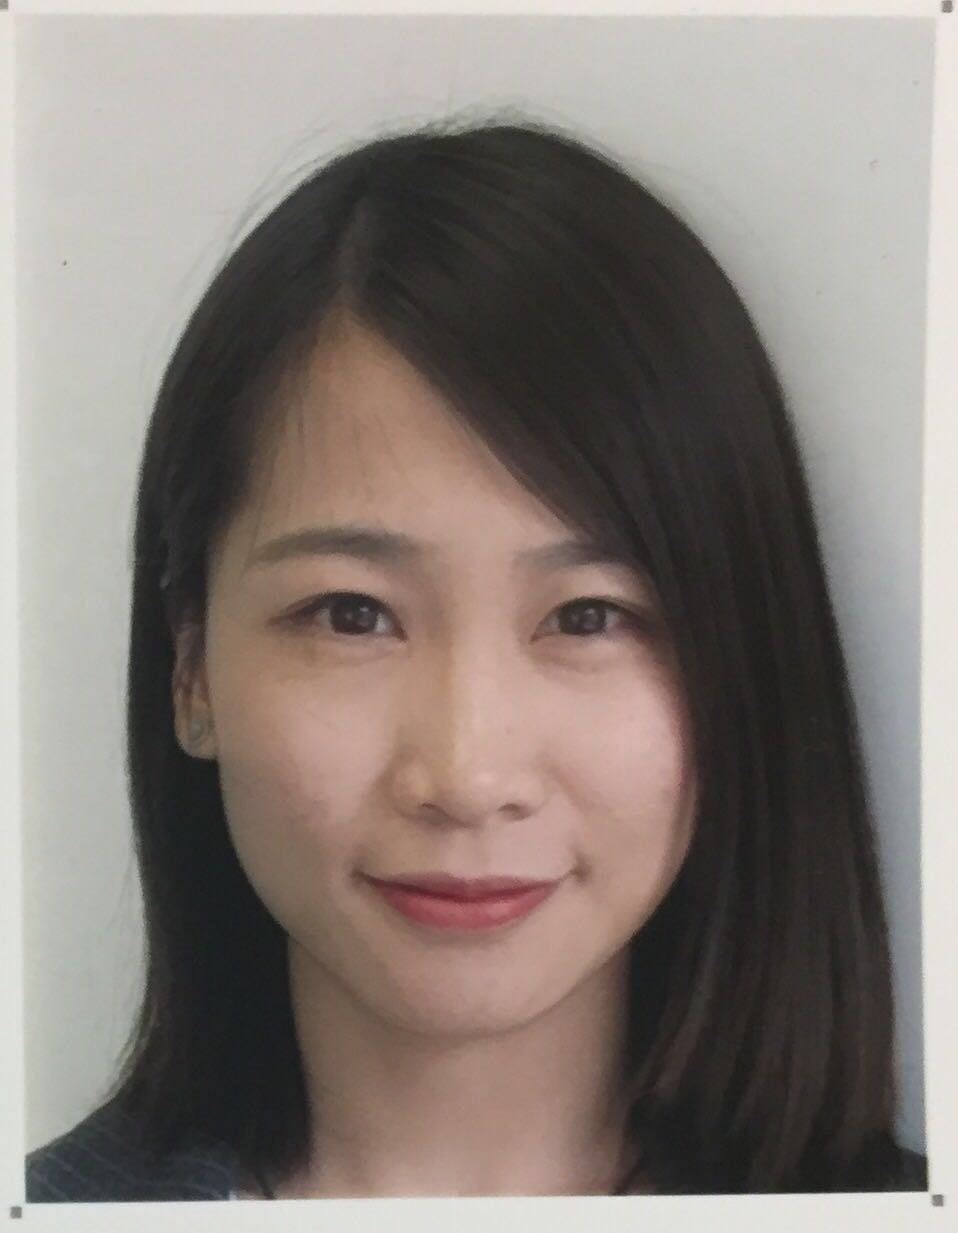
\includegraphics[width=1in,height=1.25in,clip,keepaspectratio]{./pics/Qian.jpg}}] % hier ein Foto einbinden
{Linghan Qian}
Linghan Qian received her B.Sc in Nanjing University of Science and Technology. Her BA Thesis is about Hovering control of an UAV based on sonar-ranging. Since April 2016 she is further studying in Technische Universitaet Darmstadt with orientation Automation.
\end{biography}
\begin{biography}
[{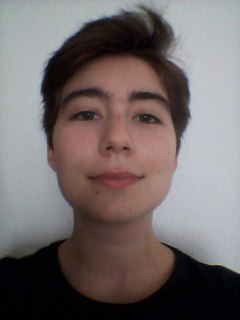
\includegraphics[width=1in,height=1.25in,clip,keepaspectratio]{./pics/Wirth.jpg}}] 
{Vivica Wirth}
received her B.~Sc. in Embedded Systems Engineernig from Albert--Ludwigs--Universität Freiburg in 2015. Her B. Sc. Thesis was about rounding edge costs on paths in graphs. Since 2015 she is studing M.~Sc. Computational Engineering at TU--Darmstadt, in 2016 she also took up M.~Sc. Autonome Systeme.

\end{biography}

\end{document}
